% Options for packages loaded elsewhere
\PassOptionsToPackage{unicode}{hyperref}
\PassOptionsToPackage{hyphens}{url}
%
\documentclass[
  a4paper,
]{article}
\usepackage{lmodern}
\usepackage{amssymb,amsmath}
\usepackage{ifxetex,ifluatex}
\ifnum 0\ifxetex 1\fi\ifluatex 1\fi=0 % if pdftex
  \usepackage[T1]{fontenc}
  \usepackage[utf8]{inputenc}
  \usepackage{textcomp} % provide euro and other symbols
\else % if luatex or xetex
  \usepackage{unicode-math}
  \defaultfontfeatures{Scale=MatchLowercase}
  \defaultfontfeatures[\rmfamily]{Ligatures=TeX,Scale=1}
\fi
% Use upquote if available, for straight quotes in verbatim environments
\IfFileExists{upquote.sty}{\usepackage{upquote}}{}
\IfFileExists{microtype.sty}{% use microtype if available
  \usepackage[]{microtype}
  \UseMicrotypeSet[protrusion]{basicmath} % disable protrusion for tt fonts
}{}
\makeatletter
\@ifundefined{KOMAClassName}{% if non-KOMA class
  \IfFileExists{parskip.sty}{%
    \usepackage{parskip}
  }{% else
    \setlength{\parindent}{0pt}
    \setlength{\parskip}{6pt plus 2pt minus 1pt}}
}{% if KOMA class
  \KOMAoptions{parskip=half}}
\makeatother
\usepackage{xcolor}
\IfFileExists{xurl.sty}{\usepackage{xurl}}{} % add URL line breaks if available
\IfFileExists{bookmark.sty}{\usepackage{bookmark}}{\usepackage{hyperref}}
\hypersetup{
  pdftitle={Lab 4},
  pdfauthor={Emilio Dorigatti},
  hidelinks,
  pdfcreator={LaTeX via pandoc}}
\urlstyle{same} % disable monospaced font for URLs
\usepackage[margin=1in]{geometry}
\usepackage{color}
\usepackage{fancyvrb}
\newcommand{\VerbBar}{|}
\newcommand{\VERB}{\Verb[commandchars=\\\{\}]}
\DefineVerbatimEnvironment{Highlighting}{Verbatim}{commandchars=\\\{\}}
% Add ',fontsize=\small' for more characters per line
\usepackage{framed}
\definecolor{shadecolor}{RGB}{248,248,248}
\newenvironment{Shaded}{\begin{snugshade}}{\end{snugshade}}
\newcommand{\AlertTok}[1]{\textcolor[rgb]{0.94,0.16,0.16}{#1}}
\newcommand{\AnnotationTok}[1]{\textcolor[rgb]{0.56,0.35,0.01}{\textbf{\textit{#1}}}}
\newcommand{\AttributeTok}[1]{\textcolor[rgb]{0.77,0.63,0.00}{#1}}
\newcommand{\BaseNTok}[1]{\textcolor[rgb]{0.00,0.00,0.81}{#1}}
\newcommand{\BuiltInTok}[1]{#1}
\newcommand{\CharTok}[1]{\textcolor[rgb]{0.31,0.60,0.02}{#1}}
\newcommand{\CommentTok}[1]{\textcolor[rgb]{0.56,0.35,0.01}{\textit{#1}}}
\newcommand{\CommentVarTok}[1]{\textcolor[rgb]{0.56,0.35,0.01}{\textbf{\textit{#1}}}}
\newcommand{\ConstantTok}[1]{\textcolor[rgb]{0.00,0.00,0.00}{#1}}
\newcommand{\ControlFlowTok}[1]{\textcolor[rgb]{0.13,0.29,0.53}{\textbf{#1}}}
\newcommand{\DataTypeTok}[1]{\textcolor[rgb]{0.13,0.29,0.53}{#1}}
\newcommand{\DecValTok}[1]{\textcolor[rgb]{0.00,0.00,0.81}{#1}}
\newcommand{\DocumentationTok}[1]{\textcolor[rgb]{0.56,0.35,0.01}{\textbf{\textit{#1}}}}
\newcommand{\ErrorTok}[1]{\textcolor[rgb]{0.64,0.00,0.00}{\textbf{#1}}}
\newcommand{\ExtensionTok}[1]{#1}
\newcommand{\FloatTok}[1]{\textcolor[rgb]{0.00,0.00,0.81}{#1}}
\newcommand{\FunctionTok}[1]{\textcolor[rgb]{0.00,0.00,0.00}{#1}}
\newcommand{\ImportTok}[1]{#1}
\newcommand{\InformationTok}[1]{\textcolor[rgb]{0.56,0.35,0.01}{\textbf{\textit{#1}}}}
\newcommand{\KeywordTok}[1]{\textcolor[rgb]{0.13,0.29,0.53}{\textbf{#1}}}
\newcommand{\NormalTok}[1]{#1}
\newcommand{\OperatorTok}[1]{\textcolor[rgb]{0.81,0.36,0.00}{\textbf{#1}}}
\newcommand{\OtherTok}[1]{\textcolor[rgb]{0.56,0.35,0.01}{#1}}
\newcommand{\PreprocessorTok}[1]{\textcolor[rgb]{0.56,0.35,0.01}{\textit{#1}}}
\newcommand{\RegionMarkerTok}[1]{#1}
\newcommand{\SpecialCharTok}[1]{\textcolor[rgb]{0.00,0.00,0.00}{#1}}
\newcommand{\SpecialStringTok}[1]{\textcolor[rgb]{0.31,0.60,0.02}{#1}}
\newcommand{\StringTok}[1]{\textcolor[rgb]{0.31,0.60,0.02}{#1}}
\newcommand{\VariableTok}[1]{\textcolor[rgb]{0.00,0.00,0.00}{#1}}
\newcommand{\VerbatimStringTok}[1]{\textcolor[rgb]{0.31,0.60,0.02}{#1}}
\newcommand{\WarningTok}[1]{\textcolor[rgb]{0.56,0.35,0.01}{\textbf{\textit{#1}}}}
\usepackage{graphicx}
\makeatletter
\def\maxwidth{\ifdim\Gin@nat@width>\linewidth\linewidth\else\Gin@nat@width\fi}
\def\maxheight{\ifdim\Gin@nat@height>\textheight\textheight\else\Gin@nat@height\fi}
\makeatother
% Scale images if necessary, so that they will not overflow the page
% margins by default, and it is still possible to overwrite the defaults
% using explicit options in \includegraphics[width, height, ...]{}
\setkeys{Gin}{width=\maxwidth,height=\maxheight,keepaspectratio}
% Set default figure placement to htbp
\makeatletter
\def\fps@figure{htbp}
\makeatother
\setlength{\emergencystretch}{3em} % prevent overfull lines
\providecommand{\tightlist}{%
  \setlength{\itemsep}{0pt}\setlength{\parskip}{0pt}}
\setcounter{secnumdepth}{-\maxdimen} % remove section numbering
\usepackage{bbold}
\ifluatex
  \usepackage{selnolig}  % disable illegal ligatures
\fi

\title{Lab 4}
\author{Emilio Dorigatti}
\date{2020-11-20}

\begin{document}
\maketitle

Welcome to the fourth lab. In this lab, we will derive the
backpropagation equations, code the training procedure, and test it on
our beloved dataset with five points.

\hypertarget{exercise-1}{%
\subsection{Exercise 1}\label{exercise-1}}

Consider a neural network with \(L\) layers and a loss function
\(\mathcal{L}(\textbf{y},\textbf{z}^{(L)}_{\cdot,out})\). Call the
output of the \(i\)-th unit of the \(\ell\)-th layer
\(\textbf{z}^{(\ell)}_{i,out}=\sigma^{(\ell)}(\textbf{z}^{(\ell)}_{i,in})\)
with
\(\textbf{z}^{(\ell)}_{i,in}=\sum_j\textbf{W}^{(\ell)}_{ji}\textbf{z}^{(\ell-1)}_{j,out}+\textbf{b}^{(\ell)}_{i}\)
its pre-activation output. Finally, consider
\(\delta^{(\ell)}_i=\partial\mathcal{L}(\textbf{y},\textbf{z}^{(L)}_{\cdot,out})/\partial\mathbf{z}^{(\ell)}_{i,in}\)
the gradient of the loss with respect to the pre-activation outputs of
layer \(\ell\).

Derive the back-propagation algorithm for a network with arbitrary
architecture. You might find the results of the previous lab a useful
reference, as well as chapter 5 of the book \emph{Mathematics for
Machine Learning} (\url{https://mml-book.github.io}).

\begin{enumerate}
\item Show that
\begin{align}
\delta^{(L)}_i &= \frac{\partial\mathcal{L}(\textbf{y},\textbf{z}^{(L)}_{\cdot,out})}{\partial\textbf{z}^{(L)}_{i,out}}
\cdot{\sigma^\prime}^{(L)}(\textbf{z}^{(L)}_{i,in})
\\
\label{eq:dldwji}
\frac{\partial \mathcal{L}(\textbf{y},\textbf{z}^{(L)}_{\cdot,out})}{\partial \textbf{W}^{(\ell)}_{ji}}&=\delta^{(\ell)}_i\cdot\textbf{z}^{(\ell-1)}_{j,out} \\
\frac{\partial \mathcal{L}(\textbf{y},\textbf{z}^{(L)}_{\cdot,out})}{\partial \textbf{b}^{(\ell)}_{i}}&=\delta^{(\ell)}_i \\
\label{eq:deltas}
\delta^{(\ell-1)}_i&=\left(\sum_k\delta^{(\ell)}_k\cdot\textbf{W}^{(\ell)}_{ik}\right)\cdot{\sigma^\prime}^{(\ell-1)}(\textbf{z}^{(\ell-1)}_{i,in})
\end{align}

\item Use vectorized operations (i.e., operations with vectors and matrices) to compute the gradients with respect to a single sample.

\item Extend the vectorized operations to handle data in batches, and show that:
\begin{align}
\Delta^{(L)}&=\nabla_{\textbf{Z}^{(L)}_{out}}\mathcal{L}(\textbf{Y},\textbf{Z}^{(L)}_{out})\odot{\sigma^\prime}^{(L)}(\textbf{Z}^{(L)}_{in}) \\
\nabla_{\textbf{W}^{(\ell)}}\mathcal{L}(\textbf{Y},\textbf{Z}^{(\ell)}_{out})&={\textbf{Z}^{(\ell-1)}_{out}}^T \cdot\Delta^{(\ell)} \\
\nabla_{\textbf{b}^{(\ell)}}\mathcal{L}(\textbf{Y},\textbf{Z}^{(L)}_{out})&=\sum_i {\Delta^{(\ell)}_i}^T \\
\Delta^{(\ell-1)}&=\Delta^{(\ell)}{\textbf{W}^{(\ell)}}^T\odot{\sigma^\prime}^{(\ell-1)}(\textbf{Z}^{(\ell-1)}_{in})
\end{align}

where $\Delta^{(\ell)}$, $\textbf{Y}$ and $\textbf{Z}^{(\ell)}_{out}$ are matrices whose $i$-th row contain the respective vectors $\delta$, $\textbf{y}$ and $\textbf{z}^{(\ell)}_{\cdot,out}$ for the $i$-th sample in the batch, and $\odot$ is the element-wise product.
\end{enumerate}

\hypertarget{solution}{%
\subsubsection{Solution}\label{solution}}

\hypertarget{question-1}{%
\paragraph{Question 1}\label{question-1}}

By applying the chain rule, we have, for the last layer:

\begin{align}
\delta^{(L)}_i
&=\frac{\partial\mathcal{L}(\textbf{y},\textbf{z}^{(L)}_{\cdot,out})}{\partial\textbf{z}^{(L)}_{i,in}}
=\frac{\partial\mathcal{L}(\textbf{y},\textbf{z}^{(L)}_{\cdot,out})}{\partial\textbf{z}^{(L)}_{i,out}}
  \cdot\frac{\partial\textbf{z}^{(L)}_{i,out}}{\partial\textbf{z}^{(L)}_{i,in}}
=
\underbrace{
  \frac{\partial\mathcal{L}(\textbf{y},\textbf{z}^{(L)}_{\cdot,out})}{\partial\textbf{z}^{(L)}_{i,out}}
}_{\text{Loss-dependent}}\cdot{\sigma^\prime}^{(L)}(\textbf{z}^{(L)}_{i,in})
\end{align}

Where the first term depends on the loss function. Using the chain rule
again, the derivatives of the weights of a generic layer \(\ell\) are:

\begin{align}
\frac{
  \partial \mathcal{L}(\textbf{y},\textbf{z}^{(L)}_{\cdot,out})
}{
  \partial \textbf{W}^{(\ell)}_{ji}
}
&=\frac{
  \partial \mathcal{L}(\textbf{y},\textbf{z}^{(L)}_{\cdot,out})
}{
  \partial \textbf{z}^{(\ell)}_{i,in}
}\cdot\frac{
  \partial \textbf{z}^{(\ell)}_{i,in}
}{
  \partial \textbf{W}^{(\ell)}_{ji}
} \\
&=\delta^{(\ell)}_i\cdot\frac{
  \partial
}{
  \partial \textbf{W}^{(\ell)}_{ji}
}\underbrace{\left(
  \sum_k\textbf{W}^{(\ell)}_{ki}\textbf{z}^{(\ell-1)}_{k,out}+\textbf{b}^{(\ell)}_{i}
\right)}_{\textbf{z}^{(\ell)}_{i,in}} \\
&=\delta^{(\ell)}_i\cdot\textbf{z}^{(\ell-1)}_{j,out}
\end{align}

And, as for the bias:

\begin{align}
\frac{
  \partial \mathcal{L}(\textbf{y},\textbf{z}^{(L)}_{\cdot,out})
}{
    \partial \textbf{b}^{(\ell)}_{i}
}
&=\frac{
  \partial \mathcal{L}(\textbf{y},\textbf{z}^{(L)}_{\cdot,out})
}{
  \partial \textbf{z}^{(\ell)}_{i,in}
}\cdot\frac{
  \partial \textbf{z}^{(\ell)}_{i,in}
}{
  \partial \textbf{b}^{(\ell)}_{i}
} \\
&=\delta^{(\ell)}_i\cdot\frac{
  \partial
}{
  \partial \textbf{b}^{(\ell)}_{i}
}\underbrace{\left(
  \sum_k\textbf{W}^{(\ell)}_{ki}\textbf{z}^{(\ell-1)}_{k,out}+\textbf{b}^{(\ell)}_{i}
\right)}_{\textbf{z}^{(\ell)}_{i,in}} \\
&=\delta^{(\ell)}_i
\end{align}

Finally, the deltas of the previous layer are:

\begin{align}
\delta^{(\ell-1)}_i
&=\frac{
  \partial\mathcal{L}(\textbf{y},\textbf{z}^{(L)}_{\cdot,out})
}{
  \partial\mathbf{z}^{(\ell-1)}_{i,in}
} \\
&=\frac{
  \partial\mathcal{L}(\textbf{y},\textbf{z}^{(L)}_{\cdot,out})
}{
  \partial\mathbf{z}^{(\ell-1)}_{i,out}
}
\cdot\frac{
  \partial\mathbf{z}^{(\ell-1)}_{i,out}
}{
  \partial\mathbf{z}^{(\ell-1)}_{i,in}
} \\
&=\left(
  \sum_k\frac{
    \partial\mathcal{L}(\textbf{y},\textbf{z}^{(L)}_{\cdot,out})
  }{
    \partial\mathbf{z}^{(\ell)}_{k,in}
  }\cdot\frac{
    \partial\mathbf{z}^{(\ell)}_{k,in}
  }{
    \partial\mathbf{z}^{(\ell-1)}_{i,out}
  }
\right)
\cdot{\sigma^\prime}^{(\ell-1)}(\textbf{z}^{(\ell-1)}_{i,in}) \\
&=\left(
  \sum_k
  \delta^{(\ell)}_k
  \cdot\frac{
    \partial
  }{
    \partial\mathbf{z}^{(\ell-1)}_{i,out}
  }\left(
    \sum_l\textbf{W}^{(\ell)}_{lk}\textbf{z}^{(\ell-1)}_{l,out}+\textbf{b}^{(\ell)}_{k}
  \right)
\right)\cdot{\sigma^\prime}^{(\ell-1)}(\textbf{z}^{(\ell-1)}_{i,in}) \\
&=\left(
  \sum_k\delta^{(\ell)}_k\cdot\textbf{W}^{(\ell)}_{ik}
\right)\cdot{\sigma^\prime}^{(\ell-1)}(\textbf{z}^{(\ell-1)}_{i,in})
\end{align}

\hypertarget{question-2}{%
\paragraph{Question 2}\label{question-2}}

The trick to find vectorized formulas is to see how to compute the
previous equations all at the same time via matrix multiplication.
Always check the dimensionality of the matrices and vectors involved, to
make sure the shape of the result matches what it should be.

For the last deltas, each neuron is treated independently from the
others, therefore an element-wise multiplication between the two vectors
does the job:

\begin{equation}
\label{eq:lastdelta}
\begin{aligned}
\delta^{(L)}
&=\nabla_{\textbf{z}^{(L)}_{\cdot,out}}\mathcal{L}(\textbf{y},\textbf{z}^{(L)}_{\cdot,out})
\odot{\sigma^\prime}^{(L)}(\textbf{z}^{(L)}_{\cdot,in}) \\
(N^{(L)}\times 1) &= (N^{(L)}\times 1) \odot (N^{(L)}\times 1)
\end{aligned}
\end{equation}

Where the second row indicates the dimensionality, rows times columns,
of the elements involved.

To compute the gradients for the weights in Eq. \ref{eq:dldwji}, we
multiply every activation of the previous layer by every delta of the
current layer, resulting into a matrix which contains all combinations
of \(\textbf{z}^{(\ell)}_{i,out}\) times \(\delta^{(\ell)}_j\). This is
computed as an ``outer product'':

\begin{equation}
\label{eq:gradw}
\begin{aligned}
\nabla_{\textbf{W}^{(\ell)}}\mathcal{L}(\textbf{y},\textbf{z}^{(L)}_{\cdot,out})&=\textbf{z}^{(\ell-1)}_{\cdot,out}\cdot{\delta^{(\ell)}}^T \\
(N^{(\ell-1)}\times N^{(\ell)})&=(N^{(\ell-1)}\times 1)\cdot (N^{(\ell)}\times 1)^T
\end{aligned}
\end{equation}

The gradient for the biases is easy to compute:

\begin{equation}
\nabla_{\textbf{b}^{(\ell)}}\mathcal{L}(\textbf{y},\textbf{z}^{(L)}_{\cdot,out})=\delta^\ell
\end{equation}

Finally, the deltas for the previous layer:

\begin{equation}
\begin{aligned}
\label{eq:deltasvec}
\delta^{(\ell-1)}&=\left(\textbf{W}^{(\ell)}\cdot\delta^{(\ell)}\right)
\odot{\sigma^\prime}^{(\ell-1)}(\textbf{z}^{(\ell-1)}_{\cdot,in}) \\
(N^{(\ell-1)}\times 1)&=\left(
(N^{(\ell-1)}\times N^{(\ell)})\cdot(N^{(\ell)}\times 1)
\right)\odot(N^{(\ell-1)}\times 1)
\end{aligned}
\end{equation}

Which follows because the sum in Eq. \ref{eq:deltas} is the dot-product
of the \(i\)-th row of \(\textbf{W}^{(\ell)}\) with \(\delta^{(\ell)}\).
Doing this separately for each row results in the matrix-vector
multiplication \(\textbf{W}^{(\ell)}\cdot\delta^{(\ell)}\).

\hypertarget{question-3}{%
\paragraph{Question 3}\label{question-3}}

We now extend these formulas to handle batched data. Vectors become
matrices where each row contains the vector for the corresponding sample
in the batch:

\begin{itemize}
\tightlist
\item
  The sample labels become a matrix \(\textbf{Y}\), with
  \(\textbf{Y}_{ij}\) the label for the \(j\)-th output of the \(i\)-th
  sample;
\item
  The hidden activations become \(\textbf{Z}^{(\ell)}_{out}\), with
  \(\textbf{Z}^{(\ell)}_{ij,out}\) the activation of the \(j\)-th unit
  in the \(\ell\)-th layer for the \(i\)-th sample;
\item
  The deltas become a matrix \(\Delta^{(\ell)}\), where row \(i\)
  contains \(\delta^{(\ell)}\) for the \(i\)-th example in the batch.
\end{itemize}

Remember, the first thing you should do to understand these formulas is
to think at the dimensionality of the vectors and matrices involved and
make sure they match.

The delta for the output layer is:

\begin{equation}
\Delta^{(L)}
=\nabla_{\textbf{Z}^{(L)}_{out}}\mathcal{L}(\textbf{Y},\textbf{Z}^{(L)}_{out})
\odot{\sigma^\prime}^{(L)}(\textbf{Z}^{(L)}_{in})
\end{equation}

which looks the same as Eq. \ref{eq:lastdelta} above, except that now we
are using matrices instead of vectors. But the operation is the same:
element-wise multiplication.

The gradient with respect to \(\textbf{W}^{(\ell)}\) is a bit more
involved to compute, as it includes a three-dimensional tensor: the
first dimension is for the samples, the second dimension is for the
neurons of the \((\ell-1)\)-th layer, and the third dimension for the
neurons of the \(\ell\)-th layer. In other words, we are taking the
gradients in Eq. \ref{eq:gradw}, which are matrices, for each sample,
and ``stacking'' them one on top of each other to get a ``cube'' of
gradients. The element indexed by \(i,j,k\) is the derivative of the
loss of the \(i\)-th sample in the batch with respect to
\(\textbf{W}^{(\ell)}_{jk}\).

\begin{equation}
\left(\nabla_{\textbf{W}^{(\ell)}}\mathcal{L}(\textbf{Y},\textbf{Z}^{(L)}_{out})\right)_{ijk}
=\left(
  \frac{\partial \mathcal{L}(\textbf{Y},\textbf{Z}^{(L)}_{out})}{\partial \textbf{W}^{(\ell)}_{jk}}
\right)_i
=\textbf{Z}^{(\ell-1)}_{ij,out}\cdot\Delta^{(\ell)}_{ik}
\end{equation}

To find the gradient of the weights with respect to the whole batch, we
need to average this on the first dimension (the samples in the batch)
to get the gradient:

\begin{equation}
\frac{\partial\mathcal{L}(\textbf{Y},\textbf{Z}^{(L)}_{out})}{\partial \textbf{W}^{(\ell)}_{jk}}
=\sum_i
\textbf{Z}^{(\ell-1)}_{ij,out}
\cdot\Delta^{(\ell)}_{ik}
\end{equation}

If you look closely, you should realize that this is just a matrix
product. Let's use a simpler notation to make it clear:

\begin{equation}
A_{jk}=\sum_i B_{ij}\cdot C_{ik}=\sum_i {\left(B^T\right)}_{ji}\cdot C_{ik}
\end{equation}

Therefore, after much pain:

\begin{equation}
\nabla_{\textbf{W}^{(\ell)}}\mathcal{L}(\textbf{Y},\textbf{Z}^{(\ell)}_{out})
={\textbf{Z}^{(\ell-1)}_{out}}^T
\cdot\Delta^{(\ell)}
\end{equation}

The biases are straightforward, we just have to sum over the deltas of
each sample:

\begin{equation}
\nabla_{\textbf{b}^{(\ell)}}\mathcal{L}(\textbf{Y},\textbf{Z}^{(L)}_{out})=\sum_i {\Delta^{(\ell)}_i}^T
\end{equation}

Finally, the deltas of the previous layer. From Eq. \ref{eq:deltas},
each element is:

\begin{equation}
\Delta^{(\ell-1)}_{ij}=\left(
  \sum_k\Delta^{(\ell)}_{ik}\cdot\textbf{W}^{(\ell)}_{jk}
\right)\cdot{\sigma^\prime}^{(\ell-1)}(\textbf{Z}^{(\ell-1)}_{ij,in})
\end{equation}

The sum is again a matrix product, therefore:

\begin{equation}
\Delta^{(\ell-1)}=\Delta^{(\ell)}{\textbf{W}^{(\ell)}}^T\odot{\sigma^\prime}^{(\ell-1)}(\textbf{Z}^{(\ell-1)}_{in})
\end{equation}

\hypertarget{exercise-2}{%
\subsection{Exercise 2}\label{exercise-2}}

In this exercise, we will code the backpropagation algorithm and apply
it to our five-points dataset.

First, let's define a function to quickly create a neural network with
layers of given size. It will use tanh activation in the hidden layers
and sigmoid for the output layer. Although we will use it for
classification, we use the mean squared error loss for a change.

\begin{Shaded}
\begin{Highlighting}[]
\CommentTok{\# activations, losses, and their gradient}
\NormalTok{sigmoid }\OtherTok{=} \ControlFlowTok{function}\NormalTok{(x) \{ }\DecValTok{1} \SpecialCharTok{/}\NormalTok{ (}\DecValTok{1} \SpecialCharTok{+} \FunctionTok{exp}\NormalTok{(}\SpecialCharTok{{-}}\NormalTok{x)) \}}
\NormalTok{sigmoid\_derivative }\OtherTok{=} \ControlFlowTok{function}\NormalTok{(x) \{ }\FunctionTok{sigmoid}\NormalTok{(x) }\SpecialCharTok{*}\NormalTok{ (}\DecValTok{1} \SpecialCharTok{{-}} \FunctionTok{sigmoid}\NormalTok{(x)) \}}
\NormalTok{tanh\_derivative }\OtherTok{=} \ControlFlowTok{function}\NormalTok{(x) \{ }\DecValTok{1} \SpecialCharTok{{-}} \FunctionTok{tanh}\NormalTok{(x)}\SpecialCharTok{\^{}}\DecValTok{2}\NormalTok{ \}}
\NormalTok{mse }\OtherTok{=} \ControlFlowTok{function}\NormalTok{(ytrue, ypred) \{ }\FunctionTok{mean}\NormalTok{((ytrue }\SpecialCharTok{{-}}\NormalTok{ ypred)}\SpecialCharTok{\^{}}\DecValTok{2}\NormalTok{) \}}
\NormalTok{mse\_derivative }\OtherTok{=} \ControlFlowTok{function}\NormalTok{(ytrue, ypred) \{ }\DecValTok{2} \SpecialCharTok{*}\NormalTok{ (ypred }\SpecialCharTok{{-}}\NormalTok{ ytrue) }\SpecialCharTok{/} \FunctionTok{length}\NormalTok{(ytrue) \}}


\NormalTok{nnet.new }\OtherTok{=} \ControlFlowTok{function}\NormalTok{(layer\_sizes) \{}
  \CommentTok{\# all information about the network is stored in a list}
\NormalTok{  nnet }\OtherTok{=} \FunctionTok{list}\NormalTok{(}
    \AttributeTok{weights =} \FunctionTok{list}\NormalTok{(),}
    \AttributeTok{biases =} \FunctionTok{list}\NormalTok{(),}
    \AttributeTok{activations =} \FunctionTok{list}\NormalTok{(),}
    \AttributeTok{activations\_derivatives =} \FunctionTok{list}\NormalTok{(),}
    \AttributeTok{loss =}\NormalTok{ mse,}
    \AttributeTok{loss\_derivative =}\NormalTok{ mse\_derivative}
\NormalTok{  )}
  
  \CommentTok{\# create random weight matrices and bias vectors}
\NormalTok{  last\_size }\OtherTok{=}\NormalTok{ layer\_sizes[}\DecValTok{1}\NormalTok{]  }\CommentTok{\# the first element is the number of inputs}
  \ControlFlowTok{for}\NormalTok{(l }\ControlFlowTok{in} \DecValTok{2}\SpecialCharTok{:}\FunctionTok{length}\NormalTok{(layer\_sizes)) \{}
\NormalTok{    this\_size }\OtherTok{=}\NormalTok{ layer\_sizes[l]}
    
    \CommentTok{\# weights are initialize using the the famous "Glorot" initialization}
\NormalTok{    b }\OtherTok{=} \FunctionTok{sqrt}\NormalTok{(}\DecValTok{6} \SpecialCharTok{/}\NormalTok{ (this\_size }\SpecialCharTok{+}\NormalTok{ last\_size))}
\NormalTok{    nnet}\SpecialCharTok{$}\NormalTok{weights[[l }\SpecialCharTok{{-}} \DecValTok{1}\NormalTok{]] }\OtherTok{=} \FunctionTok{matrix}\NormalTok{(}
      \FunctionTok{runif}\NormalTok{(last\_size }\SpecialCharTok{*}\NormalTok{ this\_size, }\SpecialCharTok{{-}}\NormalTok{b, b), }\AttributeTok{ncol =}\NormalTok{ this\_size}
\NormalTok{    )}
    
    \CommentTok{\# biases are initialized to zero}
\NormalTok{    nnet}\SpecialCharTok{$}\NormalTok{biases[[l }\SpecialCharTok{{-}} \DecValTok{1}\NormalTok{]] }\OtherTok{=} \FunctionTok{rep}\NormalTok{(}\DecValTok{0}\NormalTok{, this\_size)}
    
    \CommentTok{\# set the activation}
\NormalTok{    nnet}\SpecialCharTok{$}\NormalTok{activations[[l }\SpecialCharTok{{-}} \DecValTok{1}\NormalTok{]] }\OtherTok{=}\NormalTok{ tanh}
\NormalTok{    nnet}\SpecialCharTok{$}\NormalTok{activations\_derivatives[[l }\SpecialCharTok{{-}} \DecValTok{1}\NormalTok{]] }\OtherTok{=}\NormalTok{ tanh\_derivative}
    
\NormalTok{    last\_size }\OtherTok{=}\NormalTok{ this\_size}
\NormalTok{  \}}
  
  \CommentTok{\# change the output activation to sigmoid}
\NormalTok{  nnet}\SpecialCharTok{$}\NormalTok{activations[[}\FunctionTok{length}\NormalTok{(nnet}\SpecialCharTok{$}\NormalTok{activations)]] }\OtherTok{=}\NormalTok{ sigmoid}
\NormalTok{  nnet}\SpecialCharTok{$}\NormalTok{activations\_derivatives[[}\FunctionTok{length}\NormalTok{(nnet}\SpecialCharTok{$}\NormalTok{activations)]] }\OtherTok{=}\NormalTok{ sigmoid\_derivative}
  
\NormalTok{  nnet}
\NormalTok{\}}

\NormalTok{nnet }\OtherTok{=} \FunctionTok{nnet.new}\NormalTok{(}\FunctionTok{c}\NormalTok{(}\DecValTok{2}\NormalTok{, }\DecValTok{5}\NormalTok{, }\DecValTok{3}\NormalTok{, }\DecValTok{1}\NormalTok{))}
\end{Highlighting}
\end{Shaded}

Let us now write the forward pass:

\begin{Shaded}
\begin{Highlighting}[]
\NormalTok{nnet.predict }\OtherTok{=} \ControlFlowTok{function}\NormalTok{(nnet, data.x) \{}
  \CommentTok{\# data.x is a matrix with samples on rows}
\NormalTok{  n\_layers }\OtherTok{=} \FunctionTok{length}\NormalTok{(nnet}\SpecialCharTok{$}\NormalTok{weights)}
\NormalTok{  zout }\OtherTok{=}\NormalTok{ data.x}
  \ControlFlowTok{for}\NormalTok{(l }\ControlFlowTok{in} \DecValTok{1}\SpecialCharTok{:}\NormalTok{n\_layers) \{}
\NormalTok{    zin }\OtherTok{=} \FunctionTok{t}\NormalTok{(}\FunctionTok{t}\NormalTok{(zout }\SpecialCharTok{\%*\%}\NormalTok{ nnet}\SpecialCharTok{$}\NormalTok{weights[[l]]) }\SpecialCharTok{+}\NormalTok{ nnet}\SpecialCharTok{$}\NormalTok{biases[[l]])}
\NormalTok{    zout }\OtherTok{=}\NormalTok{ nnet}\SpecialCharTok{$}\NormalTok{activations[[l]](zin)}
\NormalTok{  \}}
\NormalTok{  zout}
\NormalTok{\}}
\end{Highlighting}
\end{Shaded}

As in the previous labs, let us visualize the output for a randomly
initialized network:

\begin{Shaded}
\begin{Highlighting}[]
\FunctionTok{library}\NormalTok{(scales)}
\FunctionTok{library}\NormalTok{(ggplot2)}

\NormalTok{grid }\OtherTok{=} \FunctionTok{as.matrix}\NormalTok{(}\FunctionTok{expand.grid}\NormalTok{(}\AttributeTok{x1 =} \FunctionTok{seq}\NormalTok{(}\SpecialCharTok{{-}}\DecValTok{2}\NormalTok{, }\DecValTok{2}\NormalTok{, }\DecValTok{1} \SpecialCharTok{/} \DecValTok{25}\NormalTok{), }\AttributeTok{x2 =} \FunctionTok{seq}\NormalTok{(}\SpecialCharTok{{-}}\DecValTok{2}\NormalTok{, }\DecValTok{2}\NormalTok{, }\DecValTok{1} \SpecialCharTok{/} \DecValTok{25}\NormalTok{)))}
\NormalTok{plot\_grid }\OtherTok{=} \ControlFlowTok{function}\NormalTok{(predictions) \{}
  \CommentTok{\# plots the predicted value for each point on the grid;}
  \CommentTok{\# the predictions should have one column and}
  \CommentTok{\# the same number of rows (10,201) as the data}
\NormalTok{  df }\OtherTok{=} \FunctionTok{cbind}\NormalTok{(}\FunctionTok{as.data.frame}\NormalTok{(grid), }\AttributeTok{y =}\NormalTok{ predictions)}
  \FunctionTok{ggplot}\NormalTok{() }\SpecialCharTok{+}
    \FunctionTok{geom\_tile}\NormalTok{(}\FunctionTok{aes}\NormalTok{(}\AttributeTok{x =}\NormalTok{ x1, }\AttributeTok{y =}\NormalTok{ x2, }\AttributeTok{fill =}\NormalTok{ y, }\AttributeTok{color =}\NormalTok{ y), df) }\SpecialCharTok{+}
    \FunctionTok{scale\_color\_gradient2}\NormalTok{(}\AttributeTok{low =} \FunctionTok{muted}\NormalTok{(}\StringTok{"blue"}\NormalTok{, }\DecValTok{70}\NormalTok{), }\AttributeTok{mid =} \StringTok{"white"}\NormalTok{,}
                         \AttributeTok{high =} \FunctionTok{muted}\NormalTok{(}\StringTok{"red"}\NormalTok{, }\DecValTok{70}\NormalTok{), }\AttributeTok{limits =} \FunctionTok{c}\NormalTok{(}\DecValTok{0}\NormalTok{, }\DecValTok{1}\NormalTok{),}
                         \AttributeTok{midpoint =} \FloatTok{0.5}\NormalTok{) }\SpecialCharTok{+}
    \FunctionTok{scale\_fill\_gradient2}\NormalTok{(}\AttributeTok{low =} \FunctionTok{muted}\NormalTok{(}\StringTok{"blue"}\NormalTok{, }\DecValTok{70}\NormalTok{), }\AttributeTok{mid =} \StringTok{"white"}\NormalTok{,}
                        \AttributeTok{high =} \FunctionTok{muted}\NormalTok{(}\StringTok{"red"}\NormalTok{, }\DecValTok{70}\NormalTok{), }\AttributeTok{limits =} \FunctionTok{c}\NormalTok{(}\DecValTok{0}\NormalTok{, }\DecValTok{1}\NormalTok{),}
                        \AttributeTok{midpoint =} \FloatTok{0.5}\NormalTok{) }\SpecialCharTok{+}
    \FunctionTok{geom\_point}\NormalTok{(}\FunctionTok{aes}\NormalTok{(}\AttributeTok{x=}\FunctionTok{c}\NormalTok{(}\DecValTok{0}\NormalTok{, }\DecValTok{1}\NormalTok{, }\DecValTok{0}\NormalTok{, }\SpecialCharTok{{-}}\DecValTok{1}\NormalTok{, }\DecValTok{0}\NormalTok{), }\AttributeTok{y=}\FunctionTok{c}\NormalTok{(}\DecValTok{0}\NormalTok{, }\DecValTok{0}\NormalTok{, }\SpecialCharTok{{-}}\DecValTok{1}\NormalTok{, }\DecValTok{0}\NormalTok{, }\DecValTok{1}\NormalTok{)))}
\NormalTok{\}}

\CommentTok{\# run this a few times to see what different random networks predict}
\NormalTok{nnet }\OtherTok{=} \FunctionTok{nnet.new}\NormalTok{(}\FunctionTok{c}\NormalTok{(}\DecValTok{2}\NormalTok{, }\DecValTok{5}\NormalTok{, }\DecValTok{3}\NormalTok{, }\DecValTok{1}\NormalTok{))}
\FunctionTok{plot\_grid}\NormalTok{(}\FunctionTok{nnet.predict}\NormalTok{(nnet, grid))}
\end{Highlighting}
\end{Shaded}

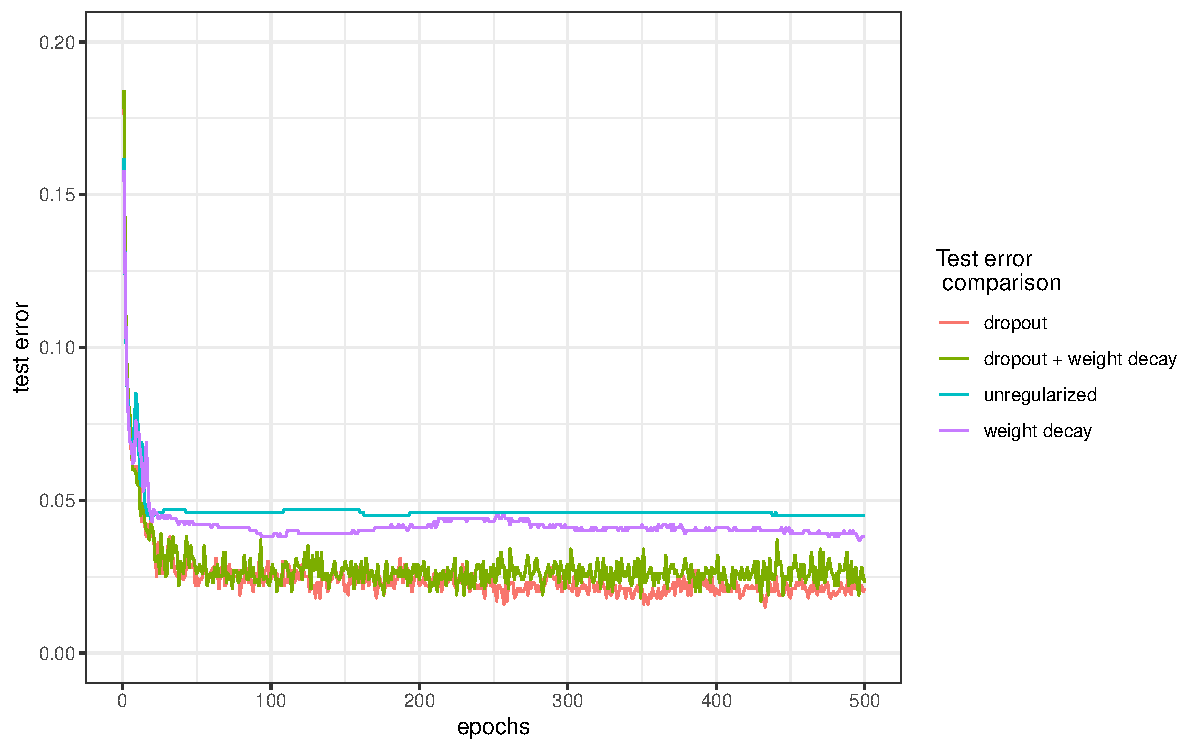
\includegraphics{lab4-solutions_files/figure-latex/unnamed-chunk-3-1.pdf}

Now, we code backpropagation to compute the gradients. Use the
vectorized formulas in Equations 5-8 to make your code much faster.

\begin{Shaded}
\begin{Highlighting}[]
\NormalTok{nnet.gradients }\OtherTok{=} \ControlFlowTok{function}\NormalTok{(nnet, x, y) \{}
  \CommentTok{\# x is be a matrix with samples on rows}
  \CommentTok{\# y is a vector with the labels}
  
\NormalTok{  n\_layers }\OtherTok{=} \FunctionTok{length}\NormalTok{(nnet}\SpecialCharTok{$}\NormalTok{weights)}
\NormalTok{  activations }\OtherTok{=} \FunctionTok{list}\NormalTok{(x)}
\NormalTok{  pre\_activations }\OtherTok{=} \FunctionTok{list}\NormalTok{(x)}
  \ControlFlowTok{for}\NormalTok{(l }\ControlFlowTok{in} \DecValTok{1}\SpecialCharTok{:}\NormalTok{n\_layers) \{}
\NormalTok{    zin }\OtherTok{=} \FunctionTok{t}\NormalTok{(}\FunctionTok{t}\NormalTok{(activations[[l]] }\SpecialCharTok{\%*\%}\NormalTok{ nnet}\SpecialCharTok{$}\NormalTok{weights[[l]]) }\SpecialCharTok{+}\NormalTok{ nnet}\SpecialCharTok{$}\NormalTok{biases[[l]])}
\NormalTok{    zout }\OtherTok{=}\NormalTok{ nnet}\SpecialCharTok{$}\NormalTok{activations[[l]](zin)}
\NormalTok{    pre\_activations[[l }\SpecialCharTok{+} \DecValTok{1}\NormalTok{]] }\OtherTok{=}\NormalTok{ zin}
\NormalTok{    activations[[l }\SpecialCharTok{+} \DecValTok{1}\NormalTok{]] }\OtherTok{=}\NormalTok{ zout}
\NormalTok{  \}}
\NormalTok{  loss }\OtherTok{=}\NormalTok{ nnet}\SpecialCharTok{$}\FunctionTok{loss}\NormalTok{(y, activations[[}\FunctionTok{length}\NormalTok{(activations)]])}
  
\NormalTok{  weights\_gradients }\OtherTok{=} \FunctionTok{list}\NormalTok{()}
\NormalTok{  biases\_gradients }\OtherTok{=} \FunctionTok{list}\NormalTok{()}
  \CommentTok{\# Eq. 5}
\NormalTok{  deltas }\OtherTok{=}\NormalTok{ nnet}\SpecialCharTok{$}\FunctionTok{loss\_derivative}\NormalTok{(}
\NormalTok{    y, activations[[}\FunctionTok{length}\NormalTok{(activations)]]}
\NormalTok{  ) }\SpecialCharTok{*}\NormalTok{ nnet}\SpecialCharTok{$}\NormalTok{activations\_derivatives[[n\_layers]](pre\_activations[[}\FunctionTok{length}\NormalTok{(activations)]])}
  \ControlFlowTok{for}\NormalTok{(l }\ControlFlowTok{in}\NormalTok{ n\_layers}\SpecialCharTok{:}\DecValTok{1}\NormalTok{) \{}
\NormalTok{    weights\_gradients[[l]] }\OtherTok{=} \FunctionTok{t}\NormalTok{(activations[[l]]) }\SpecialCharTok{\%*\%}\NormalTok{ deltas  }\CommentTok{\# Eq. 6}
\NormalTok{    biases\_gradients[[l]] }\OtherTok{=} \FunctionTok{colSums}\NormalTok{(deltas)  }\CommentTok{\# Eq. 7}
    
    \ControlFlowTok{if}\NormalTok{(l }\SpecialCharTok{\textgreater{}} \DecValTok{1}\NormalTok{) \{}
      \CommentTok{\# Eq. 8}
\NormalTok{      deltas }\OtherTok{=}\NormalTok{ deltas }\SpecialCharTok{\%*\%} \FunctionTok{t}\NormalTok{(}
\NormalTok{        nnet}\SpecialCharTok{$}\NormalTok{weights[[l]]}
\NormalTok{      ) }\SpecialCharTok{*}\NormalTok{ nnet}\SpecialCharTok{$}\NormalTok{activations\_derivatives[[l }\SpecialCharTok{{-}} \DecValTok{1}\NormalTok{]](pre\_activations[[l]])}
\NormalTok{    \}}
\NormalTok{  \}}
  
  \CommentTok{\# make sure the gradients have the correct size}
  \ControlFlowTok{for}\NormalTok{(l }\ControlFlowTok{in} \DecValTok{1}\SpecialCharTok{:}\NormalTok{n\_layers) \{}
    \FunctionTok{stopifnot}\NormalTok{(}\FunctionTok{dim}\NormalTok{(nnet}\SpecialCharTok{$}\NormalTok{weights[[l]]) }\SpecialCharTok{==} \FunctionTok{dim}\NormalTok{(weights\_gradients[[l]]))}
    \FunctionTok{stopifnot}\NormalTok{(}\FunctionTok{length}\NormalTok{(nnet}\SpecialCharTok{$}\NormalTok{biases[[l]]) }\SpecialCharTok{==} \FunctionTok{length}\NormalTok{(biases\_gradients[[l]]))}
\NormalTok{  \}}
  
  \CommentTok{\# return gradients as a list}
  \FunctionTok{list}\NormalTok{(}
    \AttributeTok{loss =}\NormalTok{ loss,}
    \AttributeTok{weights\_gradients =}\NormalTok{ weights\_gradients,}
    \AttributeTok{biases\_gradients =}\NormalTok{ biases\_gradients}
\NormalTok{  )}
\NormalTok{\}}

\NormalTok{data.x }\OtherTok{=} \FunctionTok{matrix}\NormalTok{(}\FunctionTok{c}\NormalTok{(}
  \DecValTok{0}\NormalTok{, }\DecValTok{1}\NormalTok{, }\DecValTok{0}\NormalTok{, }\SpecialCharTok{{-}}\DecValTok{1}\NormalTok{, }\DecValTok{0}\NormalTok{,}
  \DecValTok{0}\NormalTok{, }\DecValTok{0}\NormalTok{, }\SpecialCharTok{{-}}\DecValTok{1}\NormalTok{, }\DecValTok{0}\NormalTok{, }\DecValTok{1}
\NormalTok{), }\AttributeTok{ncol =} \DecValTok{2}\NormalTok{)}
\NormalTok{data.y }\OtherTok{=} \FunctionTok{c}\NormalTok{(}\DecValTok{1}\NormalTok{, }\DecValTok{0}\NormalTok{, }\DecValTok{0}\NormalTok{, }\DecValTok{0}\NormalTok{, }\DecValTok{0}\NormalTok{)}
\FunctionTok{nnet.gradients}\NormalTok{(nnet, data.x, data.y)}
\end{Highlighting}
\end{Shaded}

\begin{verbatim}
## $loss
## [1] 0.2519268
## 
## $weights_gradients
## $weights_gradients[[1]]
##               [,1]         [,2]          [,3]         [,4]          [,5]
## [1,]  0.0002038037 -0.001168316 -0.0009001711  0.001033912 -0.0009998162
## [2,] -0.0004942026  0.002546084  0.0016914546 -0.002360452  0.0011475807
## 
## $weights_gradients[[2]]
##               [,1]          [,2]        [,3]
## [1,] -0.0004482070 -6.256298e-06 0.001553982
## [2,] -0.0004780603 -8.758309e-06 0.001405281
## [3,] -0.0009479815 -1.812323e-05 0.002695238
## [4,] -0.0004711807 -7.830662e-06 0.001482008
## [5,] -0.0013276378 -2.602887e-05 0.003696342
## 
## $weights_gradients[[3]]
##             [,1]
## [1,] 0.004321912
## [2,] 0.010468581
## [3,] 0.008273765
## 
## 
## $biases_gradients
## $biases_gradients[[1]]
## [1] -0.004688995  0.032946858  0.022790616 -0.028361400  0.019991625
## 
## $biases_gradients[[2]]
## [1] -0.0198761400 -0.0002447866  0.0608179051
## 
## $biases_gradients[[3]]
## [1] 0.1480732
\end{verbatim}

We now need to implement gradient descent:

\begin{Shaded}
\begin{Highlighting}[]
\NormalTok{nnet.gradient\_descent\_step }\OtherTok{=} \ControlFlowTok{function}\NormalTok{(nnet, gradients, learning\_rate) \{}
  \ControlFlowTok{for}\NormalTok{(l }\ControlFlowTok{in} \DecValTok{1}\SpecialCharTok{:}\FunctionTok{length}\NormalTok{(nnet}\SpecialCharTok{$}\NormalTok{weights)) \{}
\NormalTok{    nnet}\SpecialCharTok{$}\NormalTok{weights[[l]] }\OtherTok{=}\NormalTok{ (}
\NormalTok{      nnet}\SpecialCharTok{$}\NormalTok{weights[[l]] }\SpecialCharTok{{-}}\NormalTok{ learning\_rate }\SpecialCharTok{*}\NormalTok{ gradients}\SpecialCharTok{$}\NormalTok{weights\_gradients[[l]]}
\NormalTok{    )}
    
\NormalTok{    nnet}\SpecialCharTok{$}\NormalTok{biases[[l]] }\OtherTok{=}\NormalTok{ (}
\NormalTok{      nnet}\SpecialCharTok{$}\NormalTok{biases[[l]] }\SpecialCharTok{{-}}\NormalTok{ learning\_rate }\SpecialCharTok{*}\NormalTok{ gradients}\SpecialCharTok{$}\NormalTok{biases\_gradients[[l]]}
\NormalTok{    )}
\NormalTok{  \}}
\NormalTok{  nnet  }\CommentTok{\# return the modified parameters}
\NormalTok{\}}


\NormalTok{nnet.train }\OtherTok{=} \ControlFlowTok{function}\NormalTok{(nnet, x, y, n\_epochs, learning\_rate) \{}
\NormalTok{  losses }\OtherTok{=} \FunctionTok{list}\NormalTok{()}
  
  \ControlFlowTok{for}\NormalTok{(e }\ControlFlowTok{in} \DecValTok{1}\SpecialCharTok{:}\NormalTok{n\_epochs) \{}
\NormalTok{    gradients }\OtherTok{=} \FunctionTok{nnet.gradients}\NormalTok{(nnet, x, y)}
\NormalTok{    nnet }\OtherTok{=} \FunctionTok{nnet.gradient\_descent\_step}\NormalTok{(nnet, gradients, learning\_rate)}
\NormalTok{    losses[[}\FunctionTok{length}\NormalTok{(losses) }\SpecialCharTok{+} \DecValTok{1}\NormalTok{]] }\OtherTok{=}\NormalTok{ gradients}\SpecialCharTok{$}\NormalTok{loss}
\NormalTok{  \}}
  
  \FunctionTok{list}\NormalTok{(}
    \AttributeTok{losses =} \FunctionTok{unlist}\NormalTok{(losses),}
    \AttributeTok{nnet =}\NormalTok{ nnet}
\NormalTok{  )}
\NormalTok{\}}
\end{Highlighting}
\end{Shaded}

Finally, let us train the network on the small dataset:

\begin{Shaded}
\begin{Highlighting}[]
\NormalTok{data.x }\OtherTok{=} \FunctionTok{matrix}\NormalTok{(}\FunctionTok{c}\NormalTok{(}
  \DecValTok{0}\NormalTok{, }\DecValTok{1}\NormalTok{, }\DecValTok{0}\NormalTok{, }\SpecialCharTok{{-}}\DecValTok{1}\NormalTok{, }\DecValTok{0}\NormalTok{,}
  \DecValTok{0}\NormalTok{, }\DecValTok{0}\NormalTok{, }\SpecialCharTok{{-}}\DecValTok{1}\NormalTok{, }\DecValTok{0}\NormalTok{, }\DecValTok{1}
\NormalTok{), }\AttributeTok{ncol =} \DecValTok{2}\NormalTok{)}
\NormalTok{data.y }\OtherTok{=} \FunctionTok{c}\NormalTok{(}\DecValTok{1}\NormalTok{, }\DecValTok{0}\NormalTok{, }\DecValTok{0}\NormalTok{, }\DecValTok{0}\NormalTok{, }\DecValTok{0}\NormalTok{)}

\NormalTok{nnet }\OtherTok{=} \FunctionTok{nnet.new}\NormalTok{(}\FunctionTok{c}\NormalTok{(}\DecValTok{2}\NormalTok{, }\DecValTok{5}\NormalTok{, }\DecValTok{3}\NormalTok{, }\DecValTok{1}\NormalTok{))}
\NormalTok{result }\OtherTok{=} \FunctionTok{nnet.train}\NormalTok{(nnet, data.x, data.y, }\DecValTok{2500}\NormalTok{, }\FloatTok{0.25}\NormalTok{)}
\FunctionTok{nnet.predict}\NormalTok{(result}\SpecialCharTok{$}\NormalTok{nnet, data.x)}
\end{Highlighting}
\end{Shaded}

\begin{verbatim}
##            [,1]
## [1,] 0.97242010
## [2,] 0.01992840
## [3,] 0.01979303
## [4,] 0.01823799
## [5,] 0.01801450
\end{verbatim}

By plotting the loss after each parameter update, we can be sure that
the network converged:

\begin{Shaded}
\begin{Highlighting}[]
\FunctionTok{plot}\NormalTok{(result}\SpecialCharTok{$}\NormalTok{losses)}
\end{Highlighting}
\end{Shaded}

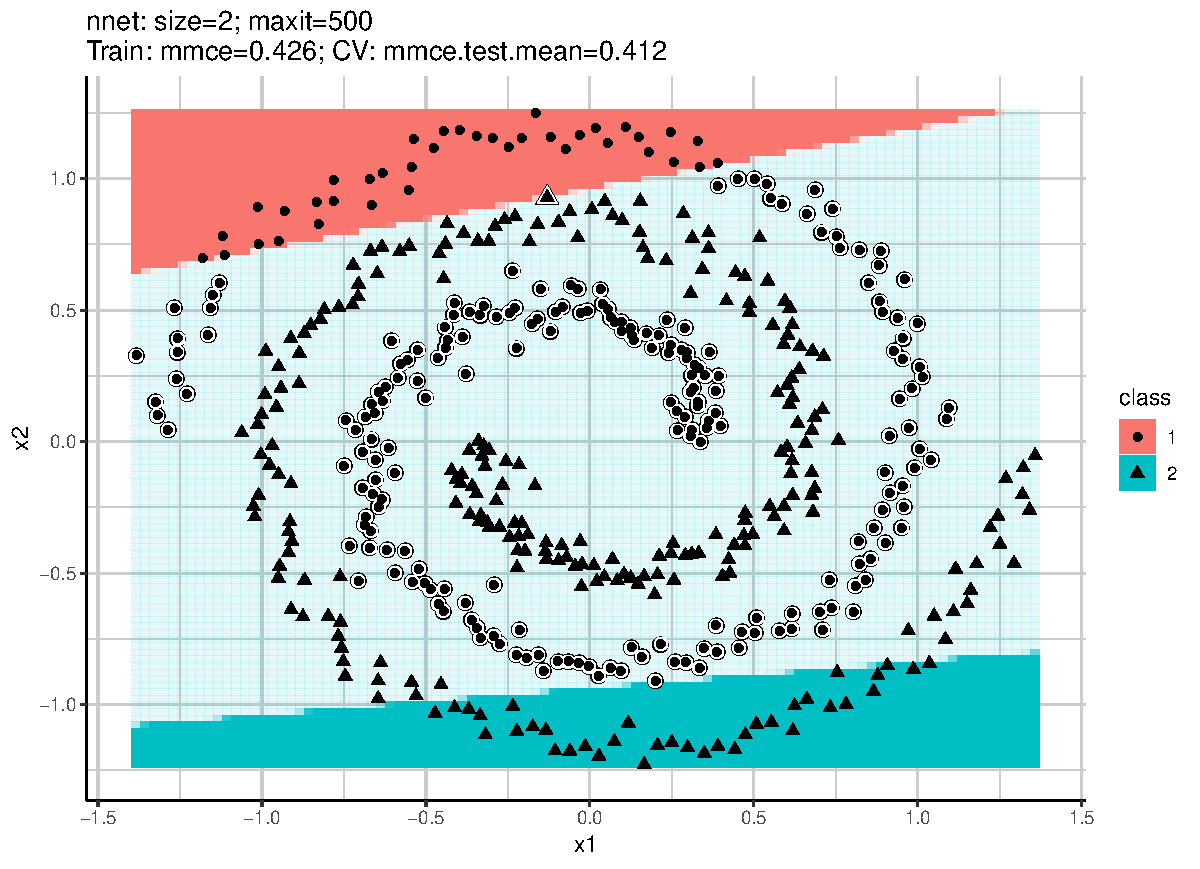
\includegraphics{lab4-solutions_files/figure-latex/unnamed-chunk-7-1.pdf}
And the decision boundary of the network is:

\begin{Shaded}
\begin{Highlighting}[]
\FunctionTok{plot\_grid}\NormalTok{(}\FunctionTok{nnet.predict}\NormalTok{(result}\SpecialCharTok{$}\NormalTok{nnet, grid))}
\end{Highlighting}
\end{Shaded}

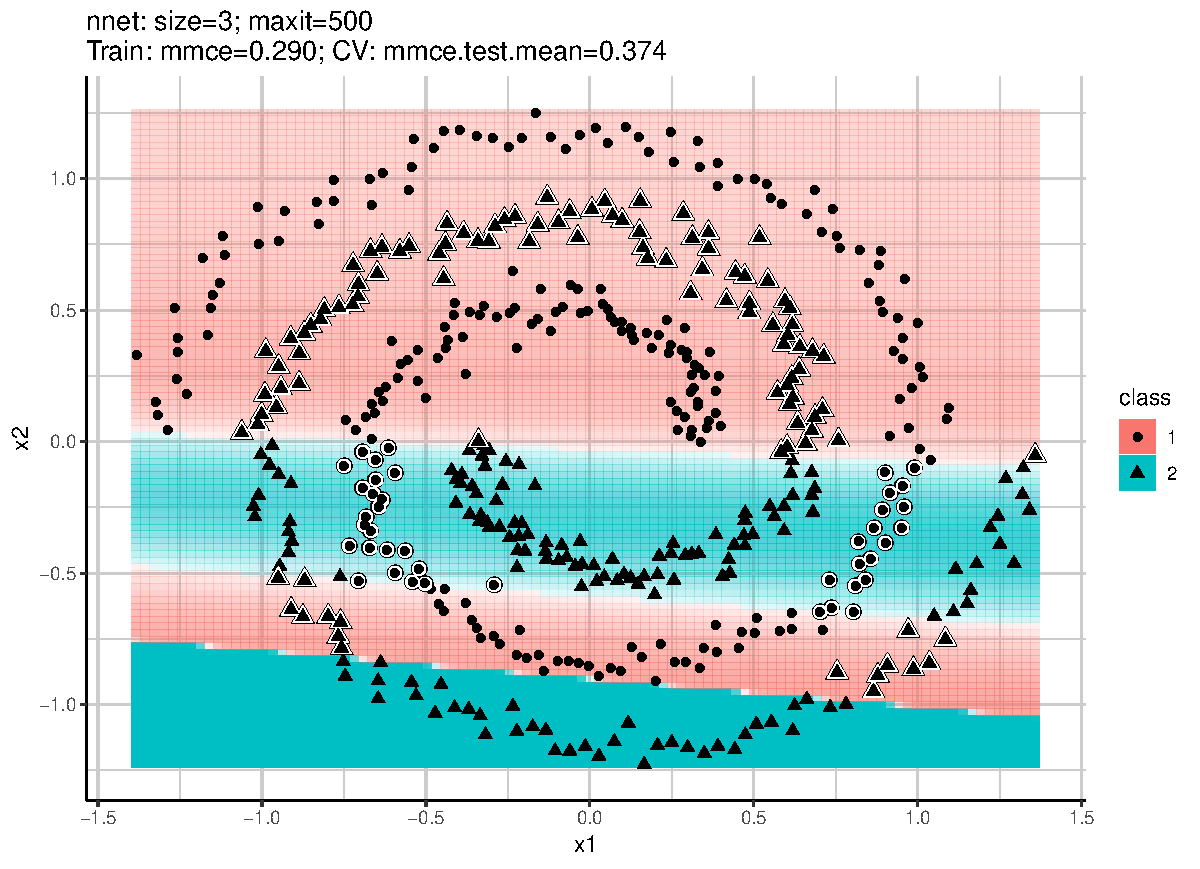
\includegraphics{lab4-solutions_files/figure-latex/unnamed-chunk-8-1.pdf}

Try to train a few randomly initialized network to discover different
decision boundaries. Try to modify the learning rate and see how it
affects the convergence speed. Finally, try different ways to initialize
the weights and note how the trainability of the network is affected.

\end{document}
